There are two different philosophies in statistics: the Classic and Bayesian. Most of the statistical formulation in this dissertation is made in Bayesian statistics, so this will be the one explained and focused. The Bayes Theorem states that:

\begin{equation}
    P(x|d) = \eta \times \frac{P(d|x)}{P(x)}
\end{equation}
\todo[inline]{Explain the meaning of Bayes theorem}

\todo[inline]{Explain Markov assumption}

Every sensor measure is noisy, so each measurement has an associated uncertainty. A common way to represent this noise is through a Gaussian or Normal distribution, which follows the following equation.

\begin{equation}
    g(x) = \frac{1}{\sigma\sqrt{2\pi}}\exp(-\frac{1}{2}\times\frac{(x - \mu)^2}{\sigma^2})
\end{equation}

\todo[inline]{Explain in 1 sentence what is a PDF}
The \acl*{PDF} for a Normal distribution takes the following shape:

\begin{figure}[H]
    \centering
    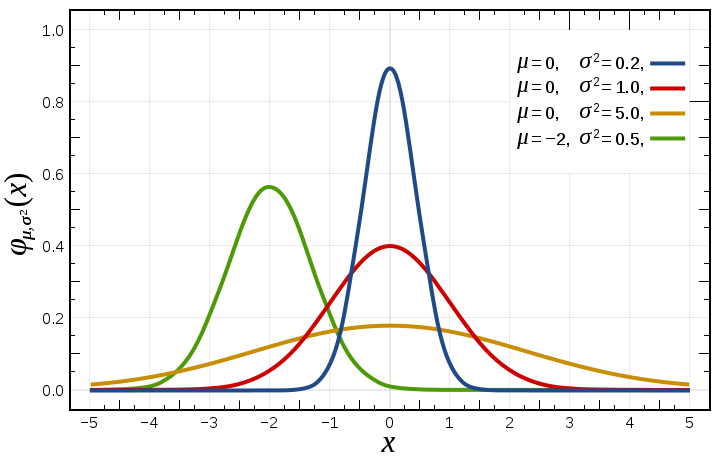
\includegraphics[width=0.5\linewidth]{images/statistics/Normal_Distribution_PDF.png}
    \caption{Normalized Gaussian curves with expected value $\mu$ and variance $\sigma^2$ \cite{enwiki:1100476982}}
    \label{fig: normal pdf}
\end{figure}

\todo[inline]{Include the picture of a gaussian distribution}

An interesting property of a Gaussian random variables is that they can be passed through a linear function and the output will also result in a gaussian variable. The result will have a different mean and \acs*{STD}. This \textbf{will not hold} for nonlinear functions. One has two different ways to solve the problem for passing a random variable through a nonlinear. The first is to locally linearize with the first order Taylor Expansion Series:

\begin{equation}
    T(x) = \sum_{n=0}^{\infty} \frac{f^{(n)}(a)}{n!}(x-a)^n
\end{equation}

\todo[inline]{Insert image of a function and Taylor Expansion}

This will make the function locally linear, but not every function will be well represented with a first order expansion. Other problem is that to compute the first Taylor expansion, one must calculate heavy jacobians, which makes the process complex/heavy/slow.
The other method is to pass several values of the initial random variable through the nonlinear function, for instance, consider the function:

\begin{equation}
    y(x) = 3x^3 + 2x^2 + x
\end{equation}

and we can compute $y(\mu)$, $y(\mu+\sigma)$, $y(\mu-\sigma)$, $y(\mu+2\sigma)$, $y(\mu-2\sigma)$, etc... if the considered $x$ values are around the mean we can compute the mean and \acs*{STD} of the y from these values. This will make $y$ a gaussian random variable. This is called an \textbf{Unscented Transform}


\section{Kalman Filters}

\todo[inline]{Explain assumptions needed}

\todo[inline]{Explain the workflow of the algorithm}

\section{Particle Filters}